\documentclass[11pt]{article}
% default ORG mode 
\usepackage[utf8]{inputenc}  \usepackage[T1]{fontenc} \usepackage{fixltx2e}
\usepackage{graphicx}        \usepackage{longtable}   \usepackage{float}
\usepackage{wrapfig}         \usepackage{soul}        \usepackage{textcomp}
\usepackage{marvosym}        \usepackage{wasysym}     \usepackage{latexsym}
\usepackage{amsmath}         \usepackage{amssymb}     \usepackage{color}
\usepackage{rotating}        \usepackage{hyperref}    \usepackage{xcolor} 
% my customizations
\definecolor{dark-red}{rgb}{0.4,0.15,0.15} 
\definecolor{dark-blue}{rgb}{0.15,0.15,0.4} 
\definecolor{medium-blue}{rgb}{0,0,0.5} 
\hypersetup{ colorlinks, linkcolor={dark-red}, citecolor={dark-blue}, urlcolor={medium-blue} }
\tolerance=1000
%\providecommand{\alert}[1]{\textbf{#1}}
\usepackage[top=1.5in, bottom=1.5in, left=1in, right=1in]{geometry}
\newcommand{\sup}[1]{^{\mbox{\scriptsize #1}}}
\newcommand{\sub}[1]{_{\mbox{\scriptsize #1}}}
\usepackage{grffile}
\DeclareGraphicsExtensions{.pdf,.png,.jpg}

\title{D\&P II.3.9a: Affine map on a convex subset}
\author{Peter Mao}
\date{\today}

\begin{document}

\maketitle

%\vspace*{1cm}

\begin{abstract}
  Exercise II.3.9a of Dodson and Poston asks us to consider an affine
  map on a convex subset of a space and prove that, when seen as a
  restriction on a map on the entire space, the larger map is unique
  if and only if the affine hull of the subset is the entire space.
  In this note, I characterize the maps that restrict to the map on
  the subset when the hull of the subset is a proper affine subspace
  of the entire set.
\end{abstract}


\section{A solution to Exercise II.3.9a of D\&P?}
\begin{quote}
Any affine map $A$ between convex sets $P \subseteq X, Q \subseteq Y$
is the restriction of an affine map $\bar{A} : X \rightarrow Y$, and
$\bar{A}$ is uniquely fixed by $A$ if and only if $H(P) = X$.
\end{quote}

At the cost of some loss of generality, let us assume that $\dim Q \le
\dim P \le \dim X = \dim Y $.\footnote{In fact, as pointed out by Joe
  and Noah, $\dim Y < \dim X$ is possible, and $\dim Y = 0$ is a
  special case.}  In a quick look at this problem, we see that $H(P) =
X$ when $\dim P = \dim X$.  Clearly the ``$\Leftarrow$'' direction of
the proof is trivial: If $H(P) = X$, there is no ``wiggle room'' for
$\bar{A}$ once we have defined $A = \bar{A}|_P$.  The
``$\Rightarrow$'' direction is a bit more interesting -- if $\bar{A}$
is unique, what does that say about $\dim P$ with respect to $\dim X$?
Let's guess that $\bar{A}$ is unique up to translations in the space
$X \setminus P$, so uniqueness would imply $X \setminus P =
\emptyset$, completing the proof.  By looking at a concrete(ish)
example, we will find that the non-uniqueness of $\bar{A}$ is a little
more interesting than my initial hand-wavy guess.

\section{A concrete example}

Following Berger (Geometry I, Chapter 2), when we pick a basis, we can
represent the affine transformation $\bar{A}: X \rightarrow Y$ with a
$(n+1)\times(n+1)$ matrix, where $n = \dim X$:
\begin{equation}\label{Eqn:Abar}
  \bar{A} = \left[
    \begin{matrix}
      1          & \mathbf{0}  \\ 
      \mathbf{y_0} & \mathbf{\bar{A}}
    \end{matrix}
  \right].
\end{equation}
In this representation, $\mathbf{y_0} \in Y$ is the $n$ dimensional
translation vector, and $\mathbf{\bar{A}}$ is the ``linear part'' of
$\bar{A}$.  For some $\mathbf{x} \in X$,
\begin{equation}\label{Eqn:AbarX}
  \bar{A}\left[ \begin{matrix} 1 \\ \mathbf{x}              \end{matrix}\right] =
         \left[ \begin{matrix} 1 \\ \mathbf{y_0 + \bar{A}x} \end{matrix}\right],
\end{equation}
so we see explicitly that $\bar{A}: \mathbf{x} \mapsto \mathbf{y_0 +
  \bar{A}x}$, in the way affine transformations do.

Now, suppose that the convex subset $P$ has lower dimensionality than
$X$.  More explicitly, let $P$ be a convex subset of the
$X$-hyperplane at some constant $x_3 = p_3$, and let $Q$ be a convex
subset of the $Y$-hyperplane at $y_1 = q_1$, as in
Figure~\ref{Fig:PQ}.  Finally, let the mapping $A: P \rightarrow Q$ be
represented by
\begin{equation}
  A = \left[
    \begin{matrix}
      1   & 0 & 0 \\
      v_2 & a & b \\
      v_3 & c & d
    \end{matrix}
    \right]
\end{equation}
so for any $\left[
  \begin{matrix}
    x_1 \\ x_2
  \end{matrix}
  \right] \in P$,
\begin{equation}\label{Eqn:A}
  \left[
    \begin{matrix}
      v_2 + ax_1 + bx_2 \\
      v_3 + cx_1 + dx_2 \\
    \end{matrix} \right] =
  \left[
    \begin{matrix}
      y_2 \\ y_3
    \end{matrix} \right] \in Q
\end{equation}

\begin{figure}[t]
\centerline{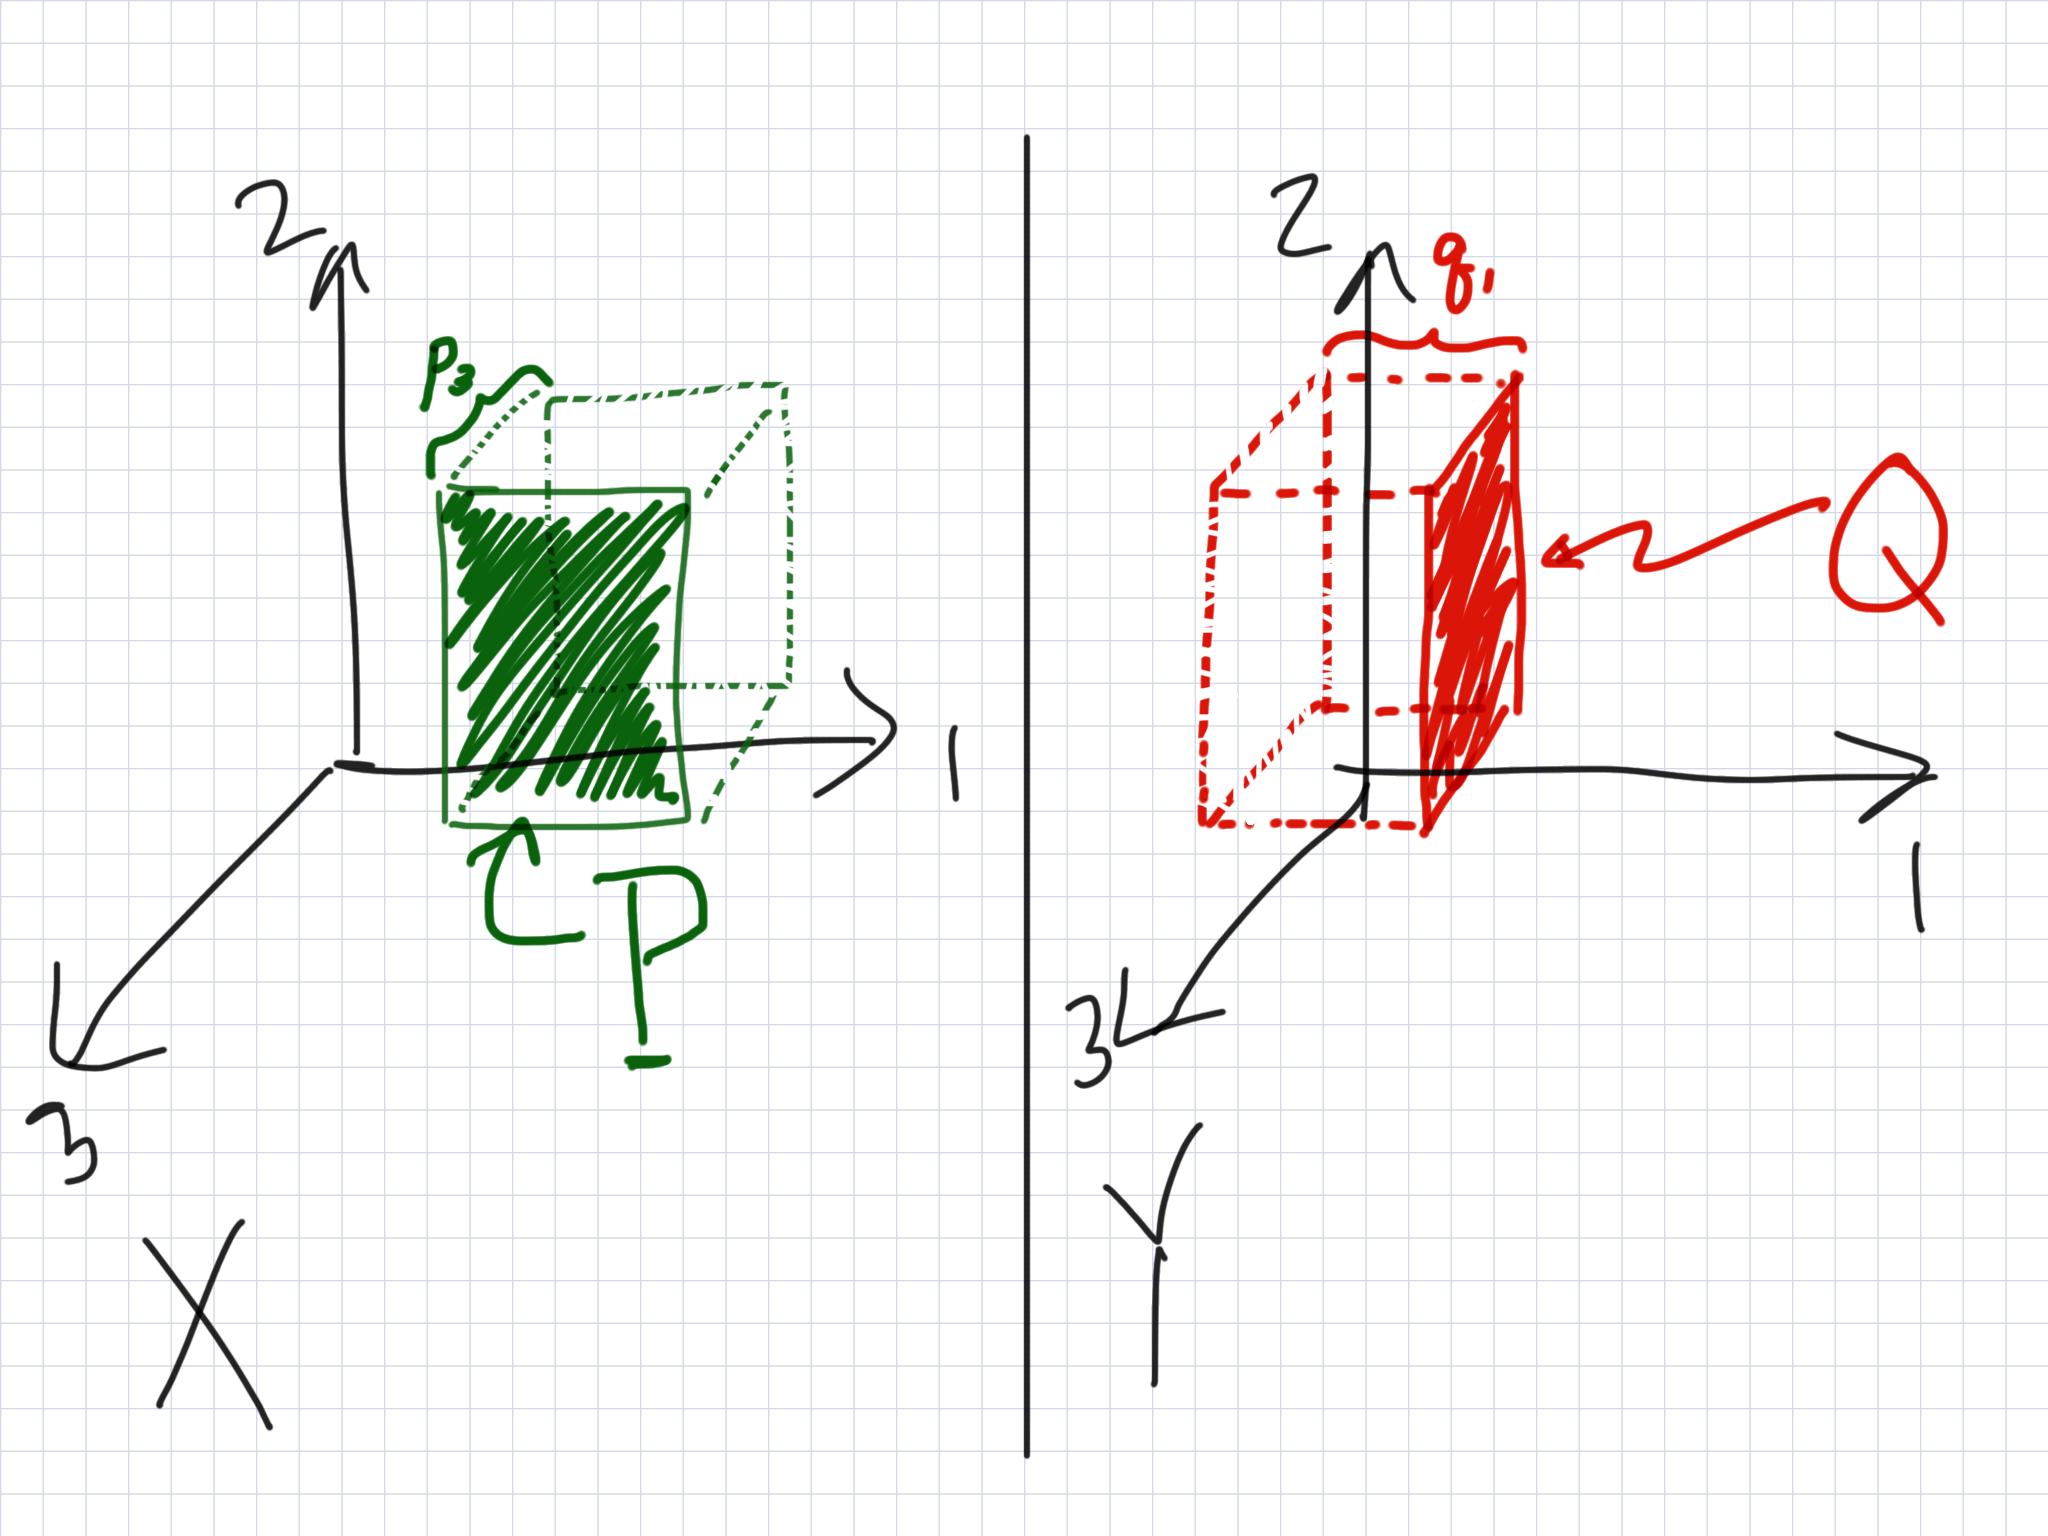
\includegraphics[height=3.25in]{DP_II.3.9a_PHM_fig1.png}}
\caption{\small The convex subsets \protect{$P \subset X$} and
  \protect{$Q \subset Y$} (in ``bird's eye axonometric'' projection).}
\label{Fig:PQ}
\end{figure}


Given $A$, what does $\bar{A}$ look like?  With no constraints,
$\bar{A}$ maps elements in $X$ to $Y$ by the rule:
\begin{equation}
  \left[ 
    \begin{matrix}
      x_1\\x_2\\x_3
    \end{matrix}
  \right] \longmapsto
  \left[
    \begin{matrix}
           1     & 0 & 0 & 0 \\
      \bar{v}_1  & \bar{r} & \bar{s} & \bar{t} \\
      \bar{v}_2  & \bar{a} & \bar{b} & \bar{u} \\
      \bar{v}_3  & \bar{c} & \bar{d} & \bar{w} 
    \end{matrix}
  \right]
  \left[
    \begin{matrix}
      1\\x_1\\x_2\\x_3
    \end{matrix}
  \right] = 
  \left[
    \begin{matrix}
      1\\y_1\\y_2\\y_3
    \end{matrix}
  \right].
\end{equation}
Restricting $\bar{A}$ to $P$ means that we only feed the matrix
$\bar{A}$ with arguments of the form
\begin{equation}
  \mathbf{x} = \left[
    \begin{matrix}
      x_1\\x_2\\p_3
    \end{matrix}
  \right],
\end{equation}
where $p_3$ is a constant.
For $A$ to be the restriction of $\bar{A}$ to $P$, the mapping must
send every element of $P$ to an element of $Q$, which looks like
\begin{equation}
  \mathbf{y} = \left[
    \begin{matrix}
      q_1\\y_2\\y_3
    \end{matrix}
  \right],
\end{equation}
where $q_1$ is the constant that defines the the location of $Q$ in $Y$.

Now, we are in a position to see characterize the nonuniqueness of
$\bar{A}$ when $\dim P < \dim X$.  Given the restriction to $P$ and
the requirement that $\bar{A}|_P: P \rightarrow Q$, we have:
\begin{equation}\label{Eqn:Abar}
  \left[
    \begin{matrix}
           1     & 0 & 0 & 0 \\
      \bar{v}_1  & \bar{r} & \bar{s} & \bar{t} \\
      \bar{v}_2  & \bar{a} & \bar{b} & \bar{u} \\
      \bar{v}_3  & \bar{c} & \bar{d} & \bar{w} 
    \end{matrix}
  \right]
  \left[
    \begin{matrix}
      1\\x_1\\x_2\\p_3
    \end{matrix}
  \right] = 
  \left[
    \begin{matrix}
      1\\q_1\\y_2\\y_3
    \end{matrix}
  \right] =
    \left[
      \begin{matrix}
        1\\ q_1 \\
      v_2 + ax_1 + bx_2 \\
      v_3 + cx_1 + dx_2 \\
    \end{matrix} \right].
\end{equation}
Since $q_1$ is a constant and $x_1$ and $x_2$ are not, $r = s = 0$.
Also, by comparing the coefficients of $x_1$ and $x_2$ in the
equations for $y_2$ and $y_3$, we make the identifications: $\bar{a} =
a$, $\bar{b} = b$, $\bar{c} = c$, and $\bar{d} = d$.  The constants in
Equation~\ref{Eqn:Abar} give us the following relationships for the
remaining parameters in $\bar{A}$:
\begin{equation}
  \left[
    \begin{matrix}
      \bar{v}_1 + \bar{t} p_3 \\
      \bar{v}_2 + \bar{u} p_3 \\
      \bar{v}_3 + \bar{w} p_3     
    \end{matrix}
    \right] = \left[
    \begin{matrix}
      q_1 \\
      v_2 \\
      v_3  
    \end{matrix}
    \right].
\end{equation}
So the translation vector of $\bar{A}$ is, in a sense, completely
arbitrary because $t$, $u$, and $w$ of $\mathbf{\bar{A}}$ are
available as extra degrees of freedom to place the output in the
correct affine subspace of $Y$, $y_1 = q_1$, with the required
translation vector of $A$, $\left[\begin{matrix}v_2\\v_3\end{matrix}\right]$.

\section{Further remarks}

I was rather surprised by this result because I had incorrectly
assumed that only translations orthogonal to $P$ would not affect its
mapping into $Q$.  Running through the example, we find that the
nonuniqueness of $\bar{A}$ lies in all components of the translation
vector \textbf{and} the part of $\bar{A}$ that couples to $X \setminus
P$.  So much for hand waving!

\section{Trouble in paradise}

Noah pointed out that for $\dim Y = 0$, $\bar{A}$ is unique no matter
what the dimensions of $P$ and $X$ are.  In the matrix representation
for $\dim P = 2$ and $\dim X = 3$, we have
\[ A = [
  \begin{matrix}
    1 & 0 & 0
  \end{matrix}
] \] and
\[ \bar{A} = [
  \begin{matrix}
    1 & 0 & 0 & 0 
  \end{matrix}
], \] so $\bar{A}$ is uniquely defined.  This
appears to be the only exception to the statement of the problem.


\end{document}



